\chapter{Quadrotor Modeling and Control}%
\label{CH:MODELING-AND-CONTROL}

In this chapter we briefly collect and review the ``golden standards'' in quadcopter modeling and control, borrowing the formalism and the
results from~\cite{tal2020accurate, faessler2017differential, kai2017nonlinear, mellinger2011minimum, richter2016polynomial, sun2022comparative, falanga2018pampc}.
The chapter unfolds as follows, in~\secref{SEC:QUADROTOR-MODELING} we develop the quadrotor dynamical model, in~\secref{SEC:DIFFERENTIAL-FLATNESS}
we describe a very useful property of the developed model known as \emph{differential flatness}.
Then in~\secref{SEC:QUADROTOR-CONTROL} %and~\secref{SEC:TRAJECTORY-GENERATION}
we briefly describe two possible quadcopter control approaches.
%and how the reference trajectories can be generated.
This chapter is intentionally poor in terms of scientific contribution as it is meant to introduce the reader to the complex world
of quadcopter motion planning and control.

%----------------------------------------------------------------------------------------
\section{Quadrotor Modeling}%
\label{SEC:QUADROTOR-MODELING}
Let $\II = \{ e^{\II}_1, e^{\II}_2, e^{\II}_3 \}$ denotes a right-hand inertial frame stationary with respect to the earth and
such that $e^{\II}_3$ denotes the vertical direction downwards into the earth.
Let the vector $\bs{\xi} = \lp x, y, z \rp\T \in \R^3$ denotes the position of the centre of mass of the object in the frame $\II$
relative to a fixed origin $O_{\II} \in \R^3$. Let $\BB = \{ e^{\BB}_1, e^{\BB}_2, e^{\BB}_3 \}$ be a body-fixed reference frame
whose center coincides with the center of mass of the vehicle and such that $e^{\BB}_3$ is in the opposite direction of thrust generation.
The attitude of the body-fixed frame is represented by a rotation matrix $R \in SO(3) : \BB \mapsto \II$, with $SO(3)$ the Special Orthogonal
group of dimension $3$.
Applying the Newton-Euler equations to the system, it is possible to retrieve the translational and rotational kinematics
\begin{equation}%
\label{EQ:QUADROTOR-KINEMATICS}
    \begin{split}
        \dot{\bs{\xi}} & = \bs{v}, \\
        \dot{R} & = RS\lp \bs{\omega} \rp,
    \end{split}
\end{equation}
with $\bs{\omega} \in \R^3$ and $\bs{v} \in \R^3$ denoting the vector of coordinates of the angular velocity and the linear 
vehicle velocity with respect to $\II$, while $S\lp \bs{\omega} \rp$ denotes the skew-symmetric matrix associated with the
vector $\bs{\omega}$, and the translational and rotational dynamics
\begin{equation}%
\label{EQ:QUADROTOR-DYNAMICS}
    \begin{split}
        \dot{\bs{v}} & = m^{-1}fRe^{\II}_3 - ge^{\II}_3, \\
        \dot{\bs{\omega}} & = -S(\bs{\omega})\bs{\omega} + J^{-1}\bs{\tau},
    \end{split}
\end{equation}
with $m \in \R$ and $J \in \R^{3 \times 3}$ being the quadrotor mass and inertia matrix with respect to the frame $\BB$,
$g \in \R$ the gravity acceleration, $f \in \R$ the collective thrust generated by the four rotors, and $\bs{\tau} \in \R^3$
the torque vector expressed in the frame $\BB$.
The system inputs are the collective thrust $f$ and the torque vector $\bs{\tau}$ which are directly generated by the rotation
of the four rotors. In particular, each rotor has an angular speed $\omega_i$ and produces a force, $F_i$, and moment, $M_i$, according to
\begin{equation*}
    F_i = k_F \omega^2_i, \hspace{0.5cm} M_i = k_M \omega^2_i,
\end{equation*}
therefore the control input to the system can be expressed as
\begin{equation*}
    \begin{pmatrix}
        f \\ \tau_x \\ \tau_y \\ \tau_z
    \end{pmatrix} =
    \begin{pmatrix}
        k_F & k_F & k_F & k_F \\
        0 & k_FL & 0 & -k_FL \\
        -k_FL & 0 & k_FL & 0 \\
        k_M & -k_M & k_M & -k_M
    \end{pmatrix}
    \begin{pmatrix}
        \omega_1^2 \\ \omega_2^2 \\ \omega_3^2 \\ \omega_4^2
    \end{pmatrix},
\end{equation*}
with $L \in \R$ the distance from the axis of rotation of the rotors to the center of the quadrotor.
For further details about the modeling of the constants $k_F \in \R$ and $k_M \in \R$ the reader is referred to~\cite{kai2017nonlinear}.
Equations~\eqref{EQ:QUADROTOR-KINEMATICS} and~\eqref{EQ:QUADROTOR-DYNAMICS} express the system dynamics with the aid of the rotational
matrix $R$, the same equation can be equivalently expressed using the quaternion dynamics as
\begin{equation}%
    \label{EQ:QUATERNION-QUADROTOR-DYNAMICS}
    \begin{split}
        \dot{\bs{\xi}} & = \bs{v}, \\
        \dot{\bs{q}} & = 0.5 \Lambda(\bs{\omega})\bs{q}, \\
        \dot{\bs{v}} & = m^{-1}fR(\bs{q})e^{\II}_3 - ge^{\II}_3, \\
        \dot{\bs{\omega}} & = -S(\bs{\omega})\bs{\omega} + J^{-1}\bs{\tau},
    \end{split}
\end{equation}
with
\begin{equation*}
    R(\bs{q}) =
    \begin{pmatrix}
        1 - 2(q_y^2 + q_z^2) & 2(q_x q_y - q_z q_w) & 2(q_x q_z + q_y q_w) \\
        2(q_x q_y + q_z q_w) & 1 - 2(q_x^2 + q_z^2) & 2(q_y q_z - q_x q_w) \\
        2(q_x q_z - q_y q_w) & 2(q_y q_z + q_x q_w) & 1 - 2(q_x^2 + q_y^2)
    \end{pmatrix},
\end{equation*}
and the matrix $\Lambda \in \R^{4 \times 4}$ defined as
\begin{equation*}
    \Lambda(\bs{\omega}) = \begin{pmatrix}
        0 & -\omega_x & -\omega_y & -\omega_z \\
        \omega_x & 0 & \omega_z & -\omega_y \\
        \omega_y & -\omega_z & 0 & \omega_x \\
        \omega_z & \omega_y & -\omega_x & 0
    \end{pmatrix}.
\end{equation*}
In the aforementioned relation $\bs{q} \in \mathbb{H}$ is the normed quaternion attitude vector.
Overall the state of the system is given by the position and velocity of the center of mass and the orientation
(locally parameterized by Euler angles) and the angular velocity
\begin{equation*}
    \bs{\xx} = \lp x, y, z, v_x, v_y, v_z, \phi, \theta, \psi, \omega_x, \omega_y, \omega_z \rp\T.
\end{equation*}

%----------------------------------------------------------------------------------------
\section{Differential Flatness}%
\label{SEC:DIFFERENTIAL-FLATNESS}
In this section we recall the results of~\cite{mellinger2011minimum} showing that the quadrotor dynamics~\eqref{EQ:QUADROTOR-KINEMATICS}-\eqref{EQ:QUADROTOR-DYNAMICS}
is differentially flat~\cite{van1998real}, i.e. the states and the inputs can be written as algebraic functions of four carefully selected
flat outputs and their derivatives. This is a fundamental result as it can ease a lot the process of trajectory generation and 
optimisation, since any smooth trajectory (with reasonably bounded derivatives) in the space of flat outputs can be followed by
the underactuated quadrotor. Let $\flatoutput = \lp x, y, z, \psi \rp\T$ the selected set of flat outputs, with
$\bs{\xi} = \lp x, y, z \rp\T$ coordinates of the center of mass in the world coordinate system and with $\psi$ the yaw angle,
and define $\flatoutput(t)$ as a smooth curve in the space of flat outputs
\begin{equation*}
    \flatoutput(t) : \lps 0, T_F \rps \mapsto \R^3 \times SO(2),
\end{equation*}
then the objective is to show that the state of the system and its control inputs can be rewritten in terms of $\sigma(t)$ and its derivatives.
First of all, the position and velocity of the center of mass are simply the first three terms of $\flatoutput$ and $\dot{\flatoutput}$.
In order to reconstruct $R$ as a function of the selected flat outputs, let us define it as $R =\ ^{\II}R_{\CC}\ ^{\CC}R_{\BB}$
where $^{\II}R_{\CC}$ represents the yaw rotation to the intermediate frame $\CC$ and $^{\CC}R_{\BB}$ represents the effect of roll and pitch.
In this setting, considering~\eqqref{EQ:QUADROTOR-DYNAMICS}, we can write
\begin{equation}%
    \label{EQ:FLAT-THRUST}
    e_3^{\BB} = \frac{m}{f} \lp \ddot{\flatoutput}_x, \ddot{\flatoutput}_y, \ddot{\flatoutput}_z + g \rp,
\end{equation}
which defines the body frame $z$-axis of the quadrotor.
From the yaw angle, $\flatoutput_4 = \psi$, we can derive the unit vector
\begin{equation*}
    e_1^{\CC} = \lp \sin\lp \flatoutput_4 \rp, \cos\lp \flatoutput_4 \rp, 0 \rp\T,
\end{equation*}
while $e_1^{\BB}$ and $e_2^{\BB}$ can be determined as
\begin{equation*}
    e_2^{\BB} = \frac{e_3^{\BB} \times e_1^{\CC}}{\norm{e_3^{\BB} \times e_1^{\CC}}}, \hspace{0.5cm} e_1^{\BB} = e_2^{\BB} \times e_3^{\BB},
\end{equation*}
provided that $e_3^{\BB} \times e_1^{\CC} \ne 0$.
Finally, the rotational matrix $R$ is uniquely determined as
\begin{equation*}
    R = \lp e_1^{\BB}, e_2^{\BB}, e_3^{\BB} \rp.
\end{equation*}
Now, take the first derivative of~\eqqref{EQ:QUADROTOR-DYNAMICS}
\begin{equation*}
    \ddot{\bs{v}} = m^{-1} \lp \dot{f}e_3^{\BB} + \bs{\omega} \times f e_3^{\BB} \rp,
\end{equation*}
projecting this equation along $e_3^{\BB}$ and using the fact that $\dot{f} = e_3^{\BB} \cdot m\ddot{\bs{v}}$,
we can define the vector $\bs{h} \in \R^3$ as
\begin{equation*}
    \bs{h} = \bs{\omega} \times e_3^{\BB} = \frac{m}{f} \lp \ddot{\bs{v}} - \lp e_3^{\BB} \cdot \ddot{\bs{v}} \rp e_3^{\BB} \rp.
\end{equation*}
In this settings, $\bs{h}$ is the projection of $\frac{m}{f} \ddot{\bs{v}}$ along the $e_1^{\BB}-e_2^{\BB}$ plane.
Thus, decoposing $\bs{\omega}$ into its components $\bs{\omega} = pe_1^{\BB} + qe_2^{\BB} + re_3^{\BB}$, we can write
\begin{equation*}
    \begin{split}
        p & = - \bs{h} \cdot e_2^{\BB}, \\
        q & = \bs{h} \cdot e_1^{\BB}, \\
        r & = \dot{\flatoutput}_4 e_3^{\II} \cdot e_3^{\BB}.
    \end{split}
\end{equation*}
Finally, the components of the angular acceleration $\bs{\alpha}$ are found by computing the second of derivative of~\eqqref{EQ:QUADROTOR-DYNAMICS}
and following the same procedure as above.
Having $\flatoutput$, $\bs{\omega}$, and $\bs{\alpha}$ at hand we can exploit~\eqqref{EQ:QUADROTOR-DYNAMICS} and~\eqqref{EQ:FLAT-THRUST}
to directly compute the inputs $f$ and $\bs{\tau}$.

%----------------------------------------------------------------------------------------
\section{Quadrotor Control}%
\label{SEC:QUADROTOR-CONTROL}
The literature is cluttered with works about the stabilisation and control of aerial vehicles such as quadcopters.
In the first stage, given the unstable nature of the quadrotors, the initial works were focused on achieving stable hovering and
near-hover flights. Thanks to the small-angle assumptions in these conditions, linear control methods such as PID and LQR
demonstrate sufficiently good performance~\cite{khatoon2014pid, dong2013modeling}.
However, as increased the necessity to push these platforms toward the boundaries of their dynamical capabilities, 
these assumptions were no longer valid. In particular, the nonlinearities coming from the attitude dynamics were no longer negligible,
for this reason researchers started developing controllers based on feedback linearization~\cite{voos2009nonlinear},
backstepping~\cite{madani2006backstepping}, and geometric properties~\cite{lee2010geometric}.
Once the differential flatness property has been revealed~\cite{mellinger2011minimum}, the differential flatness-based
controller becomes the most used regulator for trajectory tracking, as it showed the best tracking performance at
relatively high speeds~\cite{faessler2017differential, tal2020accurate}.
Besides that, recently, some studies started using Model Predictive Controls (MPCs), jointly with the full quadrotor dynamics,
to compute optimal control inputs able to both stabilise the quadcopter flight and track a given reference
trajectory~\cite{bicego2020nonlinear, foehn2021time, torrente2021data}.
These methods either directly use the optimized single rotor thrust commands~\cite{bicego2020nonlinear}
or send intermediate states from the solution (such as the angular rates) to a low-level controller~\cite{foehn2021time, torrente2021data}.
A recent study~\cite{foehn2021time} demonstrates the ability of the full-model MPC with a PID low-level controller in tracking a
pre-planned race trajectory at speed up $20 m/s$ which surpasses the top speed of $12.9 m/s$ reported in~\cite{tal2020accurate} using
a differential flatness-based controller, in spite of a much larger tracking error.

In this chapter, we briefly review these two main used control techniques based on the flatness property explained in~\secref{SEC:DIFFERENTIAL-FLATNESS}
and on the MPC tool. In the particular case of the Leonardo drone contest, we employed a non-linear model predictive controller encoding
the full quadrotor dynamics~\eqref{EQ:QUATERNION-QUADROTOR-DYNAMICS}.  

\subsection{Differential Flatness-Based Controller}
Let define the errors on position and velocity as
\begin{equation*}
    \bs{\ee}_{\bs{\xi}} = \bs{\xi} - \bs{\xi}_{\text{ref}}, \hspace{0.5cm} \bs{\ee}_{\bs{v}} = \bs{v} - \bs{v}_{\text{ref}},
\end{equation*}
then the desired force vector is
\begin{equation*}
    F_{\text{des}} = - K_{\bs{\xi}} \bs{\ee}_{\bs{\xi}} - K_{\bs{v}} \bs{\ee}_{\bs{v}} + mg e_3^{\II} + m\dot{\bs{v}}_{\text{ref}},
\end{equation*}
where $K_{\bs{\xi}}$ and $K_{\bs{v}}$ are positive definite gain matrices.
In order to compute the desired force for the quadrotor, that correspond to the first input $f$, we simply project the desired
force vector onto the actual body frame $z$-axis
\begin{equation*}
    f = F_{\text{des}} \cdot e_3^{\BB}.
\end{equation*}
To determine the other three inputs, we must consider the rotation errors.
First, observe that the desired $e_3^{\BB}$ direction is along the desired thrust vector
\begin{equation*}
    e_{3_{\text{des}}}^{\BB} = \frac{F_{\text{des}}}{\norm{F_{\text{des}}}},
\end{equation*}
thus the desired rotation is given by
\begin{equation*}
    R_{\text{des}} e_3 = e_{3_{\text{des}}}^{\BB},
\end{equation*}
with $e_3 = \lp 0, 0, 1\rp\T$.
Knowing the specified yaw angle along the trajectory, $\psi(t)$, we can compute $e_{1_{\text{des}}}^{\BB}$ and
$e_{2_{\text{des}}}^{\BB}$ as
\begin{equation*}
    e_{1_{\text{des}}}^{\CC} = \lp \cos\lp \psi \rp, \sin\lp \psi \rp, 0 \rp\T,
\end{equation*}
and 
\begin{equation*}
    e_{2_{\text{des}}}^{\BB} = \frac{e_{3_{\text{des}}}^{\BB} \times e_{1_{\text{des}}}^{\CC}}{\norm{e_{3_{\text{des}}}^{\BB} \times e_{1_{\text{des}}}^{\CC}}},
    \hspace{0.5cm} e_{1_{\text{des}}}^{\BB} = e_{2_{\text{des}}}^{\BB} \times e_{3_{\text{des}}}^{\BB}.
\end{equation*}
provided that $e_{3_{\text{des}}}^{\BB} \times e_{1_{\text{des}}}^{\CC} \ne 0$.
Next, define the error in orientation
\begin{equation*}
    \bs{\ee}_{R} = 0.5 \lp R_{\text{des}}\T R - R\T R_{\text{des}} \rp^{\land},
\end{equation*}
where $R_{\text{des}} = \lp e_{1_{\text{des}}}^{\BB}, e_{2_{\text{des}}}^{\BB}, e_{3_{\text{des}}}^{\BB}\rp$ and $^{\land}$
represents the \emph{vee map} which takes elements of $so(3)$ to $\R^3$.
The angular velocity error is simply the difference between the actual and desired angular velocity in body frame
\begin{equation*}
    \bs{\ee}_{\bs{\omega}} = \bs{\omega} - \bs{\omega}_{\text{ref}},
\end{equation*}
then the desired moments can be computed as
\begin{equation*}
    \bs{\tau} = -K_R \bs{\ee}_R -K_{\bs{\omega}} \bs{\ee}_{\bs{\omega}},
\end{equation*}
where $K_R$ and $K_{\bs{\omega}}$ are diagonal gain matrices.

\subsection{Nonlinear Model Predictive Controller}
Model predictive control generates control commands by solving a finite-time Optimal Control Problem (OCP)
in a receding horizon fashion. Given a reference trajectory, the cost function is the error between the predicted states
and the reference states inside the time horizon, meaning that multiple reference points in the time horizon are used.
In order to perform numerical optimizations, we discretize the states and inputs into $N$ equal intervals over
the time horizon $\rho \in \lps t, t+h\rps$ of size $\Delta_t = h/N$ with $h$ denoting the horizon length,
yielding a constrained nonlinear optimization problem
\begin{equation*}
    \begin{split}
        \bs{\uu} = \arg \min_{\bs{\uu}} & \sum_{k=0}^{N-1} \lp \norm{\bs{\xx}_k - \bs{\xx}_{k, \text{ref}}}_{Q} + 
                                                         \norm{\bs{\uu}_k - \bs{\uu}_{k, \text{ref}}}_{R}\rp +
                                                         \norm{\bs{\xx}_N - \bs{\xx}_{N, \text{ref}}}_{Q_N}\\
        & 
        \begin{split}
        sub. to. \hspace{0.2cm} & \bs{\xx}_{k+1} = \xfun \lp \bs{\xx}_k, \bs{\uu}_k \rp, \\
        & \bs{\xx}_0 = \bs{\xx}_{\text{init}}, \\
        & \bs{\uu} \in \lps \bs{\uu}_{\text{min}}, \bs{\uu}_{\text{max}} \rps, \\ 
        & \bs{\omega} \in \lps \bs{\omega}_{\text{min}}, \bs{\omega}_{\text{max}} \rps,
        \end{split}
    \end{split}
\end{equation*}
where the state vector is defined as $\bs{\xx} = \lp \bs{\xi}\T, \bs{v}\T, \bs{q}\T, \bs{\omega}\T \rp\T$, the input
vector as $\bs{\uu} = \lp f, \bs{\tau}\T \rp\T$, and $Q$, $R$, and $Q_N$ are positive definite matrices that shape as
\begin{equation*}
    Q = \text{diag} \lp Q_{\bs{\xi}}, Q_{\bs{v}}, Q_{\bs{q}}, Q_{\bs{\omega}} \rp, \hspace{0.2cm}
    R = \text{diag} \lp Q_{f}, Q_{\bs{\tau}} \rp, \hspace{0.2cm}
    Q_N = Q.
\end{equation*}
The reference state vector $\bs{\xx}_{\text{ref}}$ and input $\bs{\uu}_{\text{ref}}$ can be obtained from a trajectory generator procedure as described in the next chaptes,
while the function $f \lp \bs{\xx}_k, \bs{\uu}_k \rp$ is the discretized version of the full nonlinear quadrotor model~\eqref{EQ:QUATERNION-QUADROTOR-DYNAMICS}.
\begin{remark}
    In the above optimization problem, the following abuse of notation is used when calculating quaternion error
    \begin{equation*}
        \bs{q} - \bs{q}_{\text{ref}} = \bs{q} \otimes \bs{q}_{\text{ref}}^{-1}
    \end{equation*}
\end{remark}
The above MPC solves the full nonlinear model of a quadrotor, instead of resorting to a cascaded structure, or linear assumptions.
The solution presented during the Leonardo drone contest resorts on this control thecnique, where the quadratic nonlinear optimization problem is solved
by a Sequential Quadratic Programming (SQP) algorithm executed in real-time.
The algorithm has been implemented using ACADO~\cite{verschueren2018towards} toolkit with qpOASES~\cite{ferreau2014qpoases} as solver.

%----------------------------------------------------------------------------------------
% \section{Trajectory Generation}%
% \label{SEC:TRAJECTORY-GENERATION}

%% TODO: Add GP-MPC Applied to Rover
% \section{Data-Driven Model Predictive Control}
% %%%%%%%%%%
% \begin{figure}[!t]
% 	\centering
% 	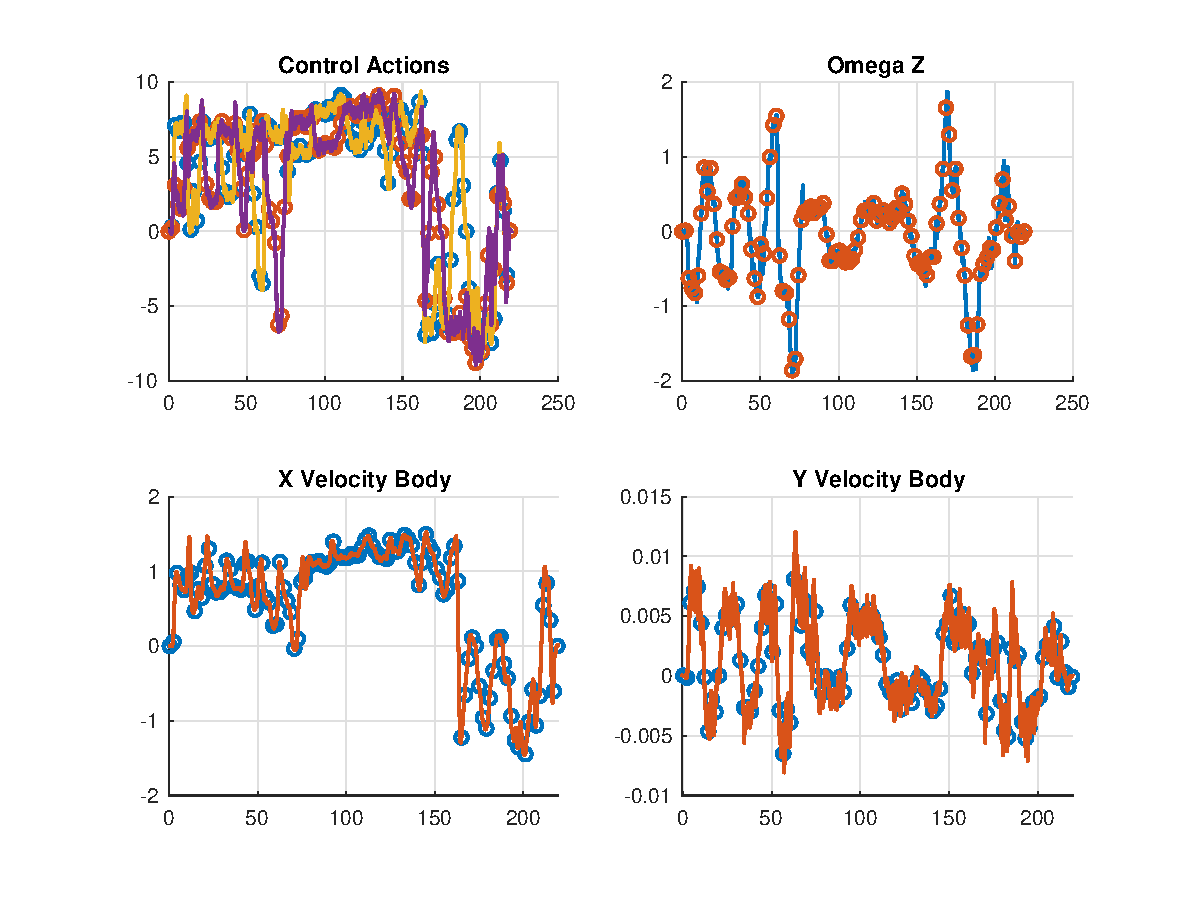
\includegraphics[width=1.\textwidth]{Figs/Chapter2/mpc_gp_sampled_quantities.eps}
% 	\caption{Caption here.}
% 	% \label{FIG:}
% \end{figure}
% %%%%%%%%%%
% %%%%%%%%%%
% \begin{figure}[!t]
% 	\centering
% 	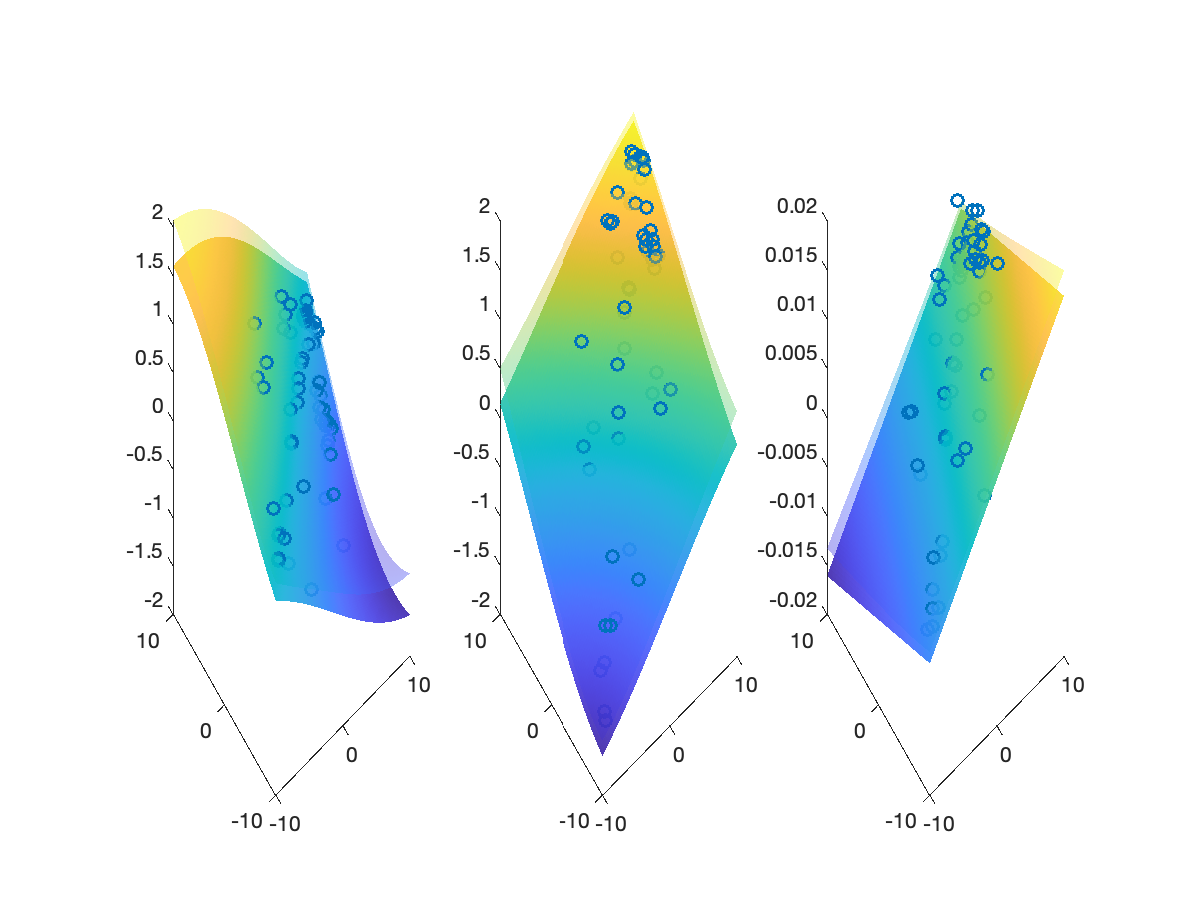
\includegraphics[width=1.\textwidth]{Figs/Chapter2/mpc_gp_regression_nl.eps}
% 	\caption{Caption here.}
% 	% \label{FIG:}
% \end{figure}
% %%%%%%%%%%
% %%%%%%%%%%
% \begin{figure}[!t]
% 	\centering
% 	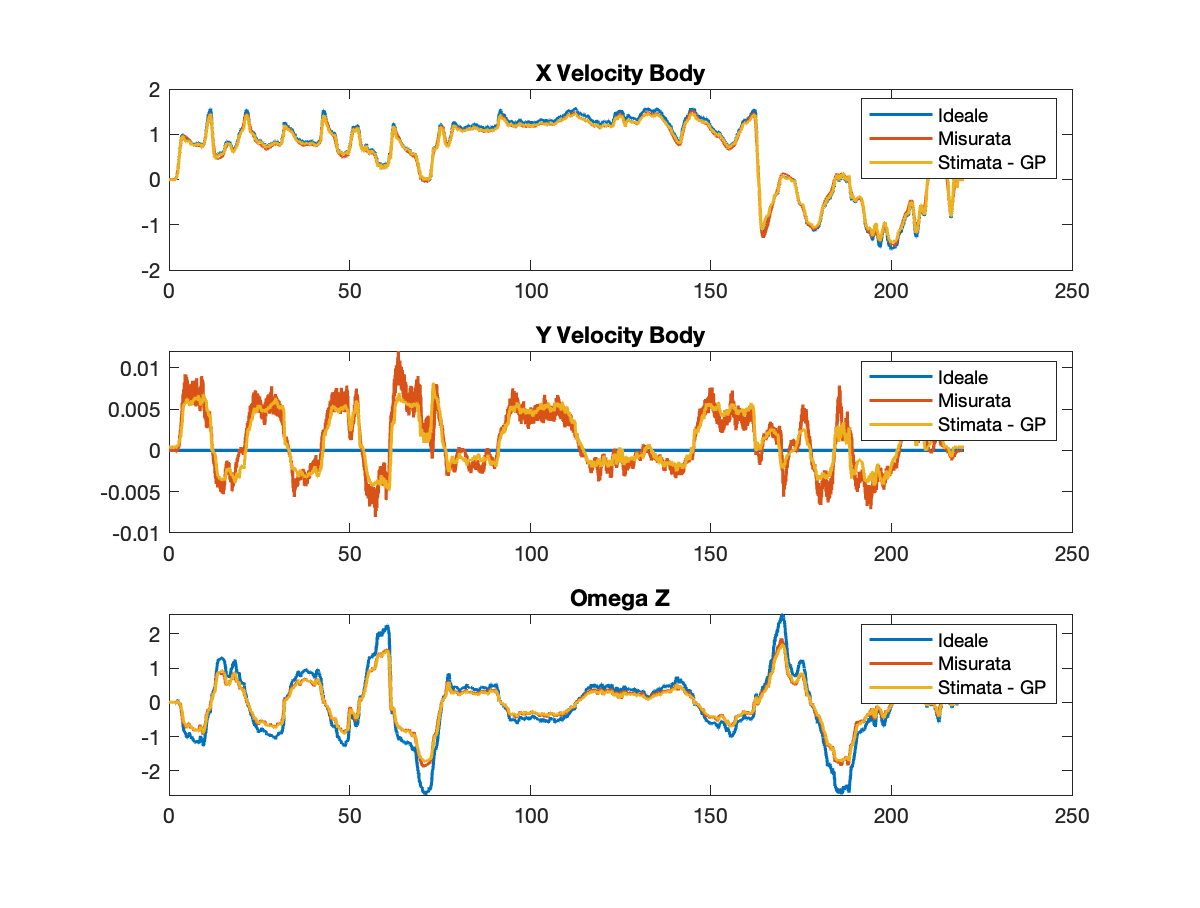
\includegraphics[width=1.\textwidth]{Figs/Chapter2/mpc_gp_test_samedata.eps}
% 	\caption{Caption here.}
% 	% \label{FIG:}
% \end{figure}
% %%%%%%%%%%
% %%%%%%%%%%
% \begin{figure}[!t]
% 	\centering
% 	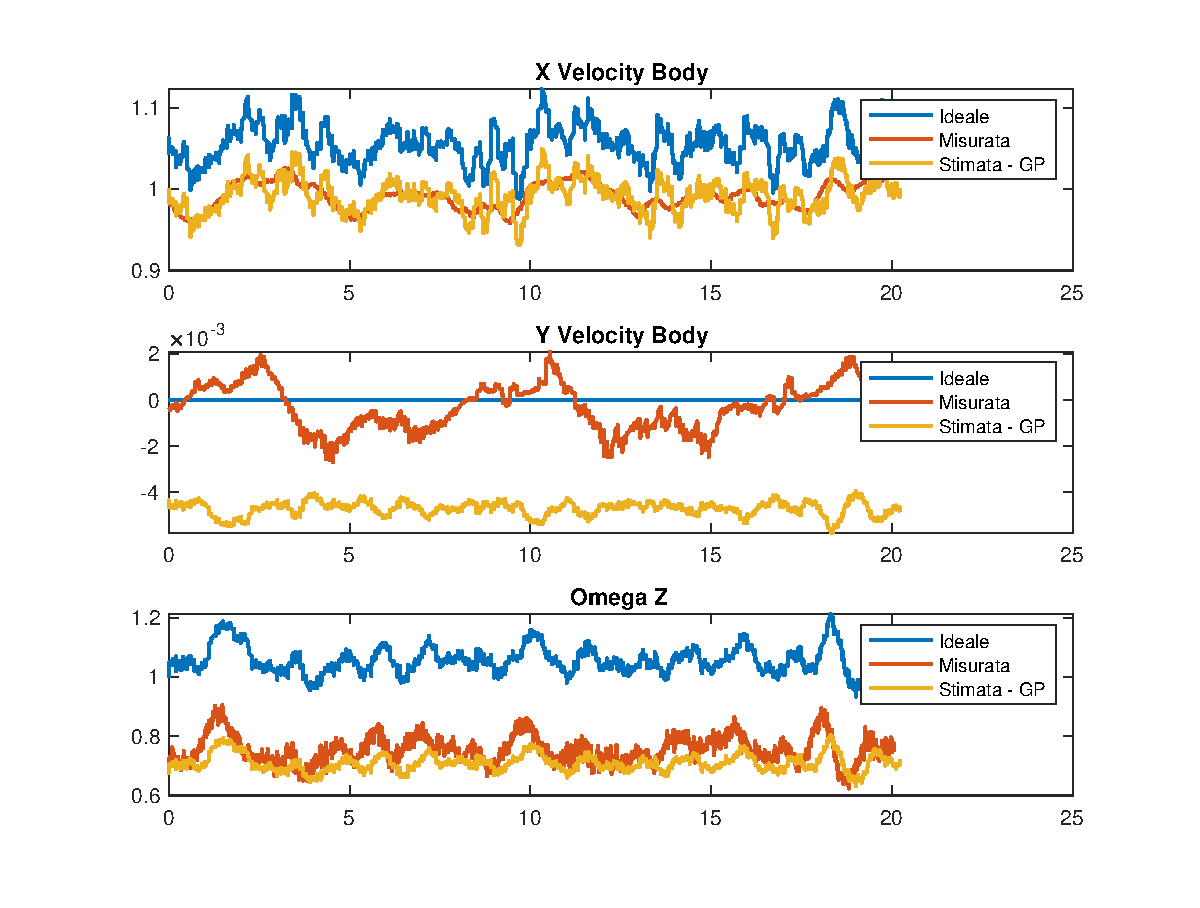
\includegraphics[width=1.\textwidth]{Figs/Chapter2/mpc_gp_test_differentdata.eps}
% 	\caption{Caption here.}
% 	% \label{FIG:}
% \end{figure}
% %%%%%%%%%%
% %%%%%%%%%%
% \begin{figure}[!t]
% 	\centering
% 	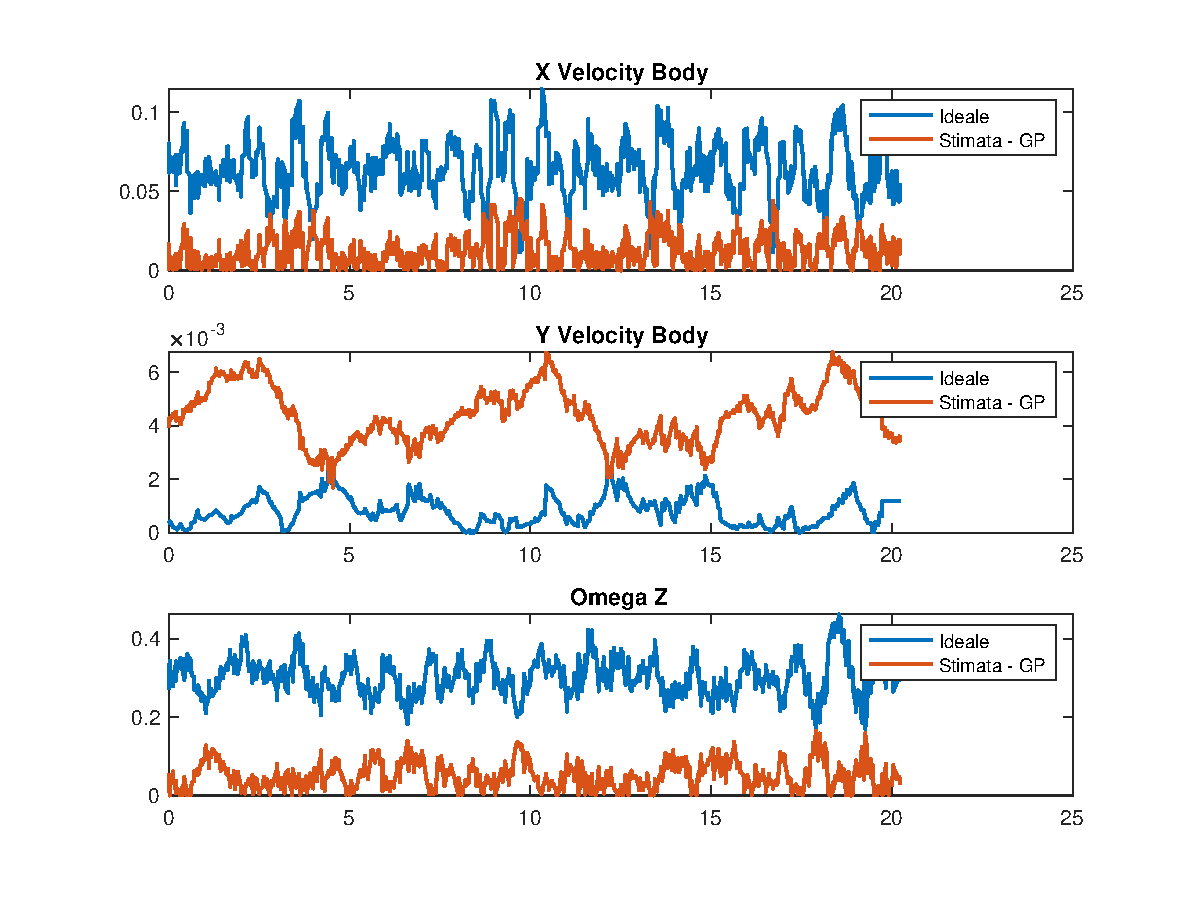
\includegraphics[width=1.\textwidth]{Figs/Chapter2/mpc_gp_test_differentdata_errors.eps}
% 	\caption{Caption here.}
% 	% \label{FIG:}
% \end{figure}
% %%%%%%%%%%

%------------------------------------------------